Research on various aspects of hovercraft design, mechanics and physics first principles, as well as input from the TA and the design decisions of our peers, led us to our own hovercraft design. This document first describes the information we uncovered about the mechanics of a hovercraft, then proceeds by describing our design and summarizing our final product.

\subsection{Hovercraft Mechanics}
The hovercraft is able to move freely due to the minimum amount of friction between the vehicle and the ground. The chamber of air between the craft and ground, called the plenum chamber, is formed by the body of the hovercraft and a skirt. The air flowing into the plenum chamber forms a ring which keeps the external lower pressure out, ensuring the persistence of the internal air cushion. The amount of air entering the plenum chamber must be at least be equal to the amount of air that escapes underneath the skirt in order to keep the craft afloat. Further, it is incorrect to assume that air will escape evenly around the skirt’s perimeter. As more air is blown into the plenum chamber, the pressure of the air on the inside becomes higher than that on the outside, creating an upward force that lifts the hovercraft. When this upward pressure exactly matches the downward force of gravity, the desired floating effect is achieved. \cite{CambridgeJournals:370274} \cite{831309}

\subsubsection{Steering}
Different approaches have been taken to steer the craft. Larger hovercrafts typically employ a large propeller at the rear to drive the vehicle forward. Rudders are used for steering. Another option, usually seen in smaller hovercrafts, is to tilt the base, affecting the plenum chamber underneath. This results in a change in direction because a drag is created on one side, creating a pivot point.


  \begin{center}
    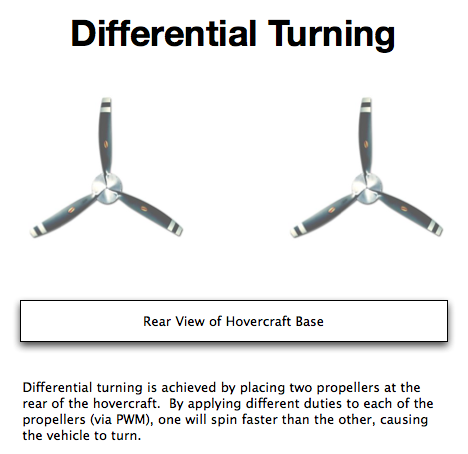
\includegraphics[width=85mm]{imageSources/differentialTurning.png}
  \end{center}
  \captionof{figure}{Differential Turning} 
  \label{differentialTurning}


Instead of using 2 fans on the craft (one for filling the plenum chamber and one for forward thrust), a single propeller may be used for both functions. A fraction of the air intake is directed into the inner chamber to lift the craft, while the remaining air flow is forced behind the craft, creating thrust.


  \begin{center}
    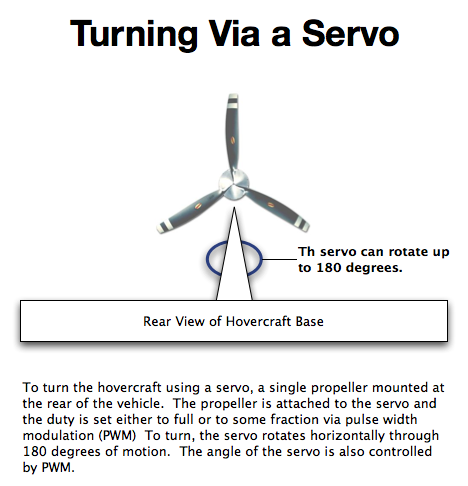
\includegraphics[width=85mm]{imageSources/servoTurning.png}
  \end{center}
  \captionof{figure}{Servo Turning} 
  \label{servoTurning}


Steering may further be affected by either differential turning or though the use of a servo motor. The former approach commonly employs two thrust sources on either side of the vehicle. By altering the thrust of either motor (for example with pulse width modulation), one motor will be more powerful than the other, causing the craft to turn. The latter approach sees a propeller mounted to a servo motor. As the servo rotates through its 180 degree range, the thrust of the propeller is directed in a specific direction, also causing the craft to turn.

\subsubsection{Skirt}
An advancement in the development of the skirt is known as the Double-Walled Flexible Skirt, or more commonly the “Big Skirt”. The design came about in the 1960’s by McReary. The idea was to inflate the outer skirt to allow the craft to move more freely over rough terrain and choppy water.

In general, the purpose of the skirt is to increase the overall surface area of the vehicle. By spreading the weight of the craft over a lager area, the pressure required to counteract this downward pressure is reduced. A common analogy is that of stepping on a single nail as opposed to lying on a bed of nails. Applying one’s entire weight on the small surface area of a single nail will surely result in a painful experience. However, by spreading one’s weight over the combined surface area of many nails, the pressure on any single point is reduced to the point where any particular nail cannot cause harm.

\subsection{Ground Effect}
Ground effect refers to the collection of aerodynamic effects felt by aircraft when flying in close proximity to the ground. If the hovercraft has too much lift, it is likely that it may well feel the effects of such a phenomenon.


  \begin{center}
    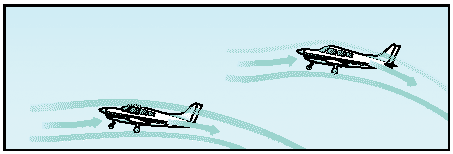
\includegraphics[width=85mm]{imageSources/groundEffect.png}
  \end{center}
  \captionof{figure}{Ground Effect Airflow} 
  \label{groundEffect}

One of the most prominent is the Wing-In-Ground effect, whereby the aircraft experiences reduced amounts of drag when flying at an altitude less than the length of its wingspan. Though the physics are somewhat complicated and beyond the scope of this report, the result is an increase in speed and lift when flying in ground effect. Ground effect is more significant for lighter aircraft than for heavier aircraft. Ground effect also has implications for rotary aircraft like helicopters. They require less energy to remain air bourn while in ground effect.

\subsection{Vortex Ring Effect}
Another interesting property of propellers, such as those used in Helicopters, is Vortex Ring effect. As helicopter blades spin, they direct air downwards, creating lift. Sometimes this air may recycle, looping around and reentering the blades. This can have a drastic effect on lift.

\begin{figure}[h]
  \begin{center}
    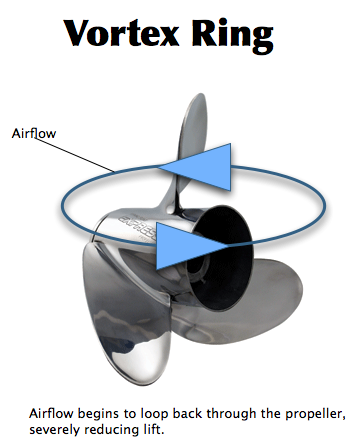
\includegraphics[width=85mm]{imageSources/vortexRing.png}
  \end{center}
  \caption{Vortex Ring Effect} 
  \label{vortexRing}
\end{figure}

\subsection{Design Schematics}

The following figures show the top, side, front and rear views for the vehicle:

\begin{figure}[h]
  \begin{center}
    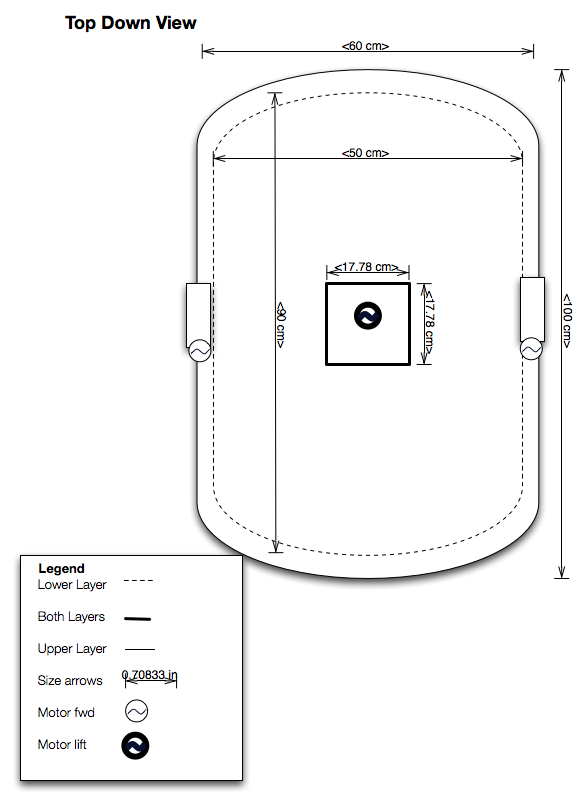
\includegraphics[width=85mm]{imageSources/topDownView.png}
  \end{center}
  \caption{Hovercraft: Top Down View} 
  \label{topDownView}
\end{figure}

The first design consisted of a rounded front, straight sides and a straight back. However, since the front and back were not symmetric, we concluded that the rear of the craft should be rounded to match the front. This symmetric design better distributes the underlying air cushion to all parts of the vehicle.

  \begin{center}
    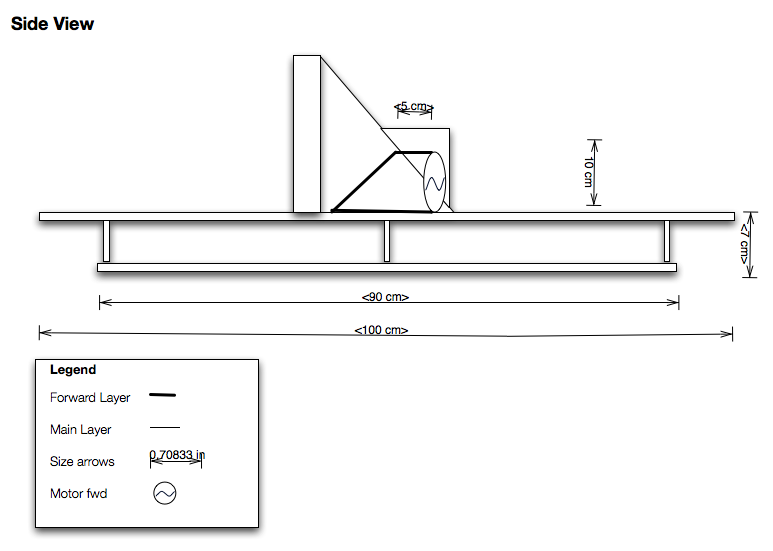
\includegraphics[width=85mm]{imageSources/sideView.png}
  \end{center}
  \caption{Hovercraft: Side View} 
  \label{sideView}

The plenum chamber receives air from a single propeller mounted in the middle of the chasis. The middle propeller is housed by a triangular container. Initially the container was completely open on the side where the propeller draws air from. We realized that too much air was escaping from this hole and a cover with a circular cut-out was fitted over the opening. The cut-out better fit the diameter of the fan, resulting in minimal air escaping from the opening.


  \begin{center}
    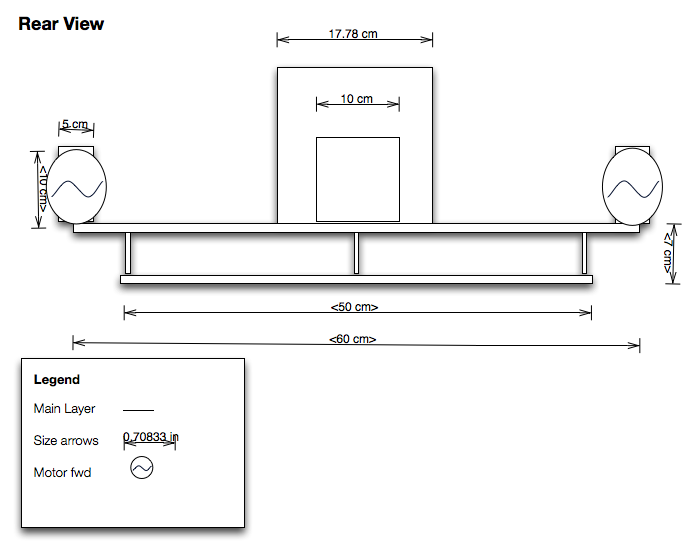
\includegraphics[width=85mm]{imageSources/rearView.png}
  \end{center}
  \caption{Hovercraft: Rear View} 
  \label{rearView}


The electronic components are mounted at the rear of the hovercraft. This facilitates making connections from the breadboard to the nearby DC Motors, servo motor, and sonars. The combined mass of all the components added a significant force to the rear of the chasis. To counter this, we placed counter weights on the front of the body.

\begin{figure}[h]
  \begin{center}
    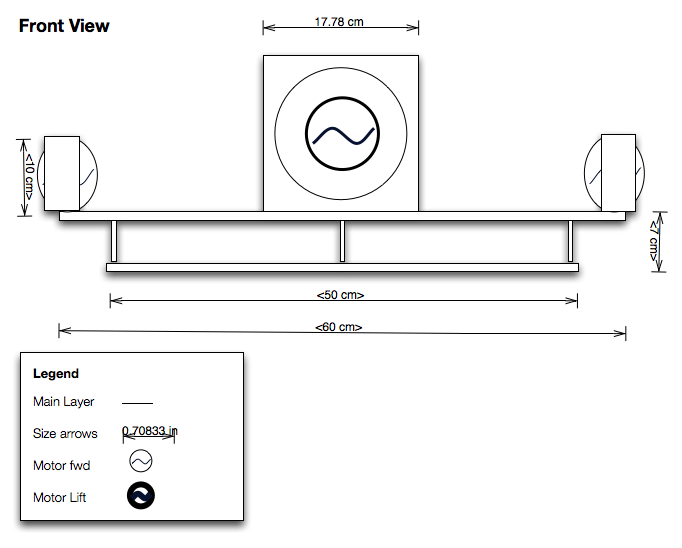
\includegraphics[width=85mm]{imageSources/frontView.png}
  \end{center}
  \caption{Hovercraft: Front View} 
  \label{frontView}
\end{figure}

\subsection{Design Constraints}
The following constraints were issues that needed to be met by the resulting hovercraft design.

\subsubsection{Payload Weight}
In order for the hovercraft to stay afloat, the internal air pressure must counter external forces placed on the surface of the vehicle by both gravity and the mass of the components. The following table describes the components and their masses:

\begin{table}
\caption{Weight of Hovercraft Components}
\begin{center}
\begin{tabular}{ c c c}
  Component & Quantity & Weight (grams) \\
  \hline
	Battery  &	2 & 	50 \\
	Breadboard &	1 &	45 \\
	Microcontroller &	1 &	15 \\
	Radio &	1 &	9 \\
	Sonar &	3 &	5 \\
	DC Motor (large) &	1 &	83 \\
	Servo Motor &	1 &	4 \\
	H-bridge &	1 &	6 \\
	DC Motor (small) &	2 &	25 \\
	Total &	-- &	329 \\
\end{tabular}
\end{center}
\label{restingTable}
\end{table}

\subsection{Rigidity}
The hovercraft body is made from two thin sheets of styrofoam separated by 12 styrofoam spacers 1'' thick. This has proven to be a very strong design, easily capable of supporting the payload of the electronics. In fact, we distributed additional weight evenly across the body and found that the hovercraft could support at least 1 kg.

\begin{figure}[h]
  \begin{center}
    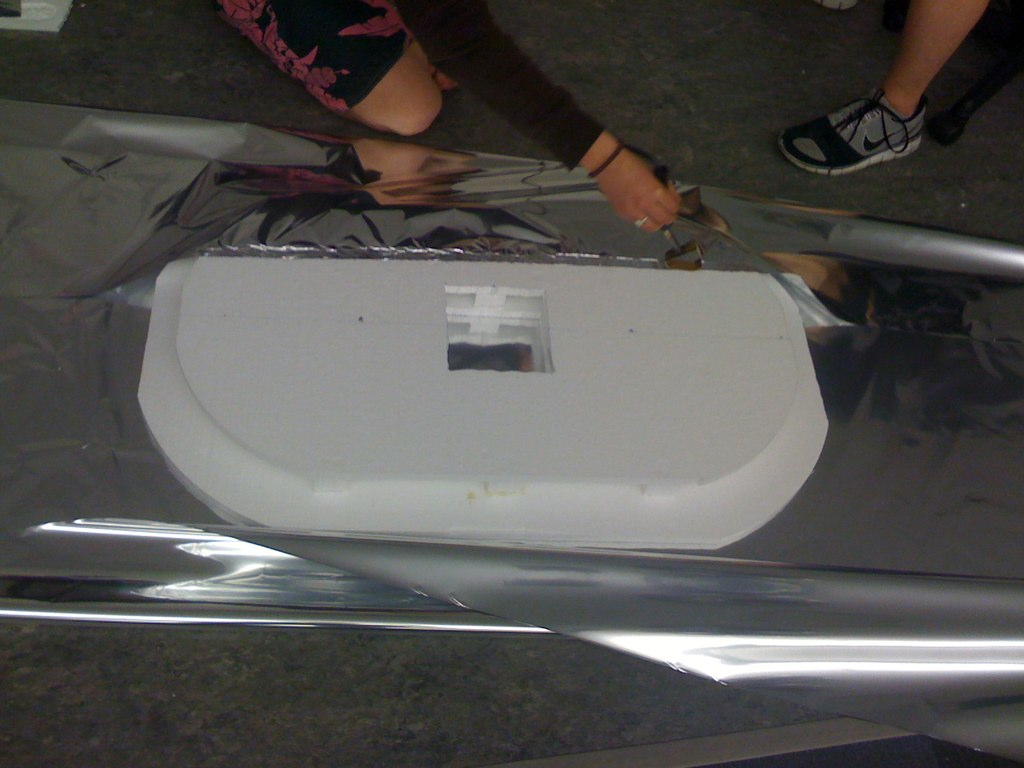
\includegraphics[width=85mm]{imageSources/rigidity1.png}
  \end{center}
  \caption{Rigidity of Hovercraft I} 
  \label{rigidity1}
\end{figure}

\begin{figure}[h]
  \begin{center}
    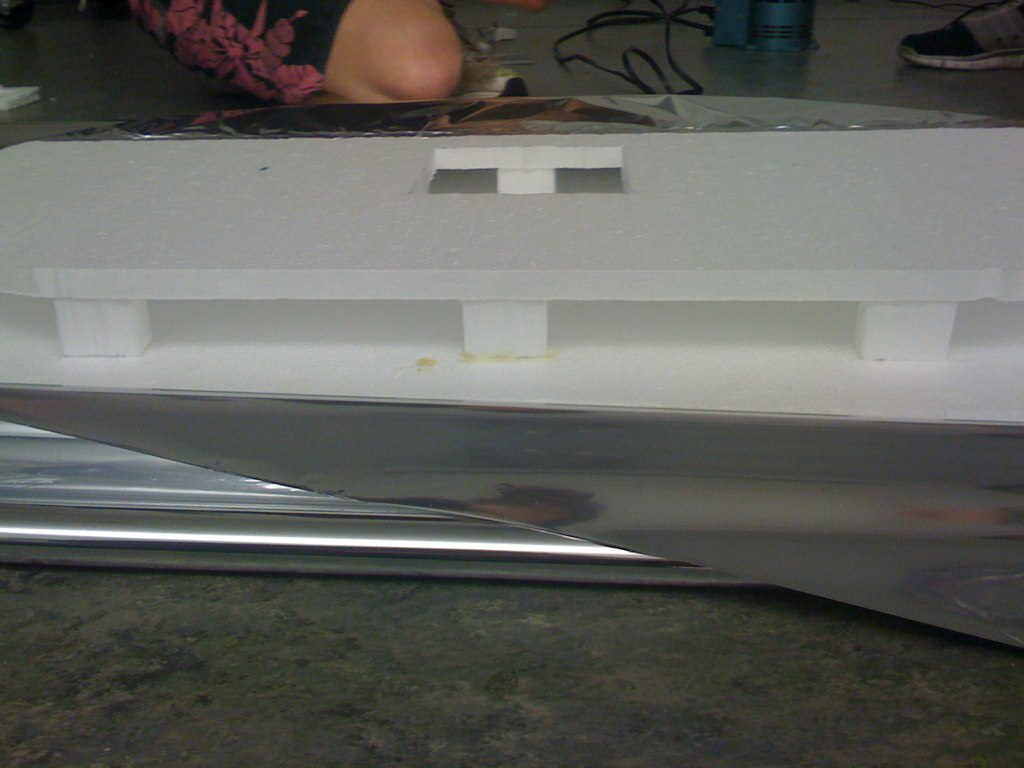
\includegraphics[width=85mm]{imageSources/rigidity2.png}
  \end{center}
  \caption{Rigidity of Hovercraft II} 
  \label{rigidity2}
\end{figure}

An inflatable skirt made of mylar surrounds the body. Mylar is a polyester film often used in flexible packaging for food, as an insulating material, and for solar reflection. Once inflated, the skirt serves two purposes. First, because it expands to over two inches, it provides additional surface area, reducing the overall pressure at any given point on the body. Second, the skirt acts as a flexible and damage resistant bumper, protecting the body from nearby objects during testing. We used two different mediums to connect the skirt to the styrofoam body. First we adhered the mylar to the styrofoam using hot glue, we then went around the perimeter with a hot iron to melt the mylar, the glue and the styrofoam together.

\begin{figure}[h]
  \begin{center}
    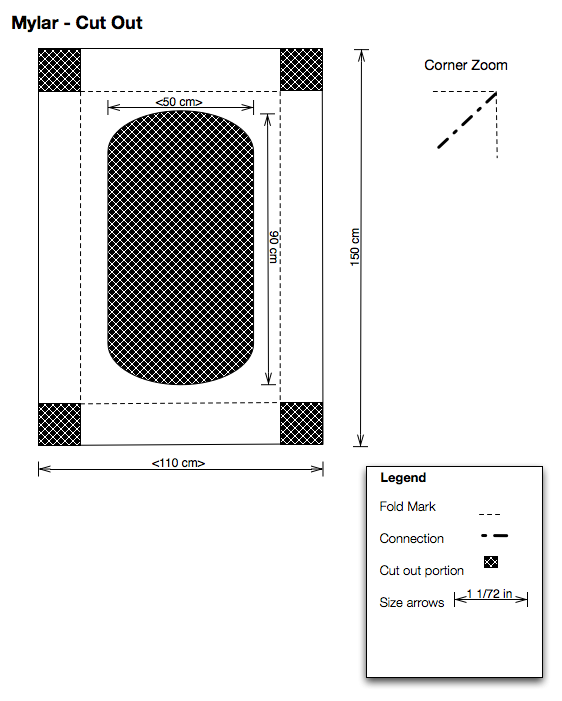
\includegraphics[width=85mm]{imageSources/mylarSchematic.png}
  \end{center}
  \caption{Schematic of the Mylar skirt} 
  \label{mylarSchematic}
\end{figure}

After the styrofoam chasis was built, we then procdeded to construct the skirt. The first attempt at constructing the mylar skirt was not successful. Lack of foresight resulted in a skirt that was too baggy in some areas, while exposing too many holes in others. The first time that we attached the mylar, when we were connecting the corners, we used clear packing tape, and simply folded the corners together. The second attempt was much more calculated and pragmatic. When connecting the corners of the second skirt, we methodically folded the edges in, then removed the square that was not attached (see Mylar-Cutout diagram). After this we made the connection using the hot iron to glue the seam together. The resulting skirt was much more evenly distributed and provided reasonably uniform inflation around the entire body. That said, the hovercraft still managed to move about when it was supposed to be idle. We addressed this issue by placing weights on the body to counteract the uneven escape of air on one side.

\subsubsection{Lift}
The decision to use a single, vertically mounted propeller to feed air into the plenum chamber was in direct response to the problem of rotational torque plaguing horizontally mounted propellers. In a horizontal design, the rotation of the blades applies an overall torque on the hovercraft causing it to spin. Dealing with this force is a burden. One approach is to install a second horizontal propeller which spins in the opposite direction. The opposite spin of the two motors cancels any directional torque felt by the craft. We chose to avoid this problem entirely by mounting a single motor vertically in the middle of the body. A container built over the propeller captures the incoming air and forces into the plenum chamber.

\begin{figure}[h]
  \begin{center}
    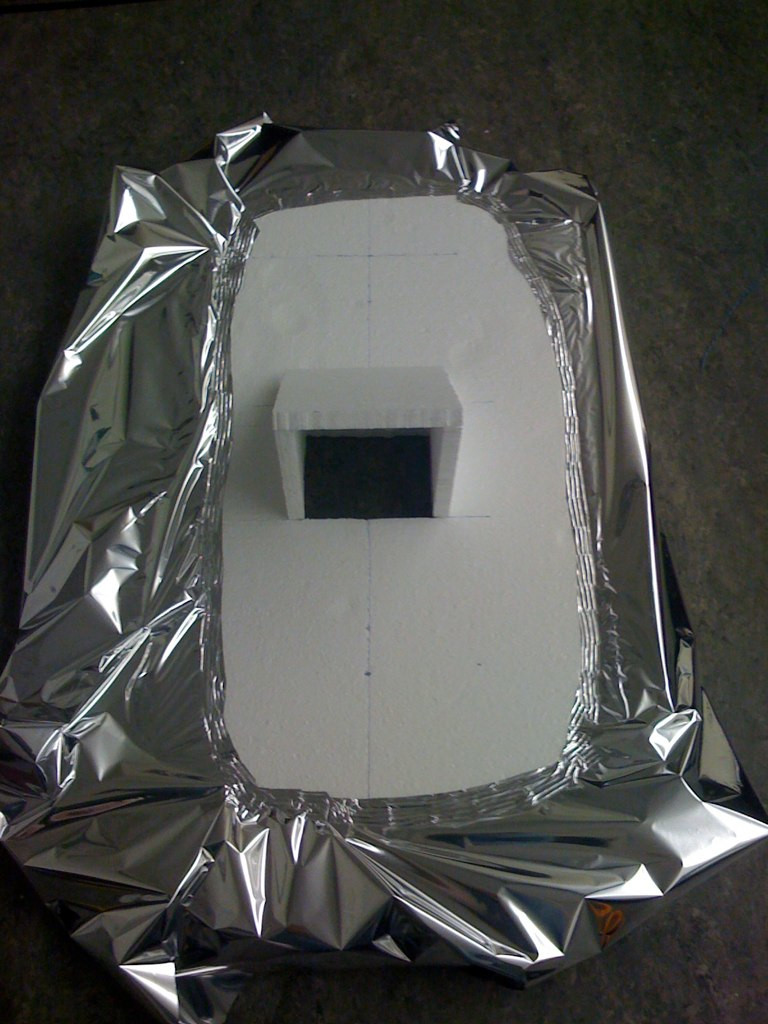
\includegraphics[width=85mm]{imageSources/lift1.png}
  \end{center}
  \caption{Hovercraft Lift I} 
  \label{lif1}
\end{figure}

\begin{figure}[h]
  \begin{center}
    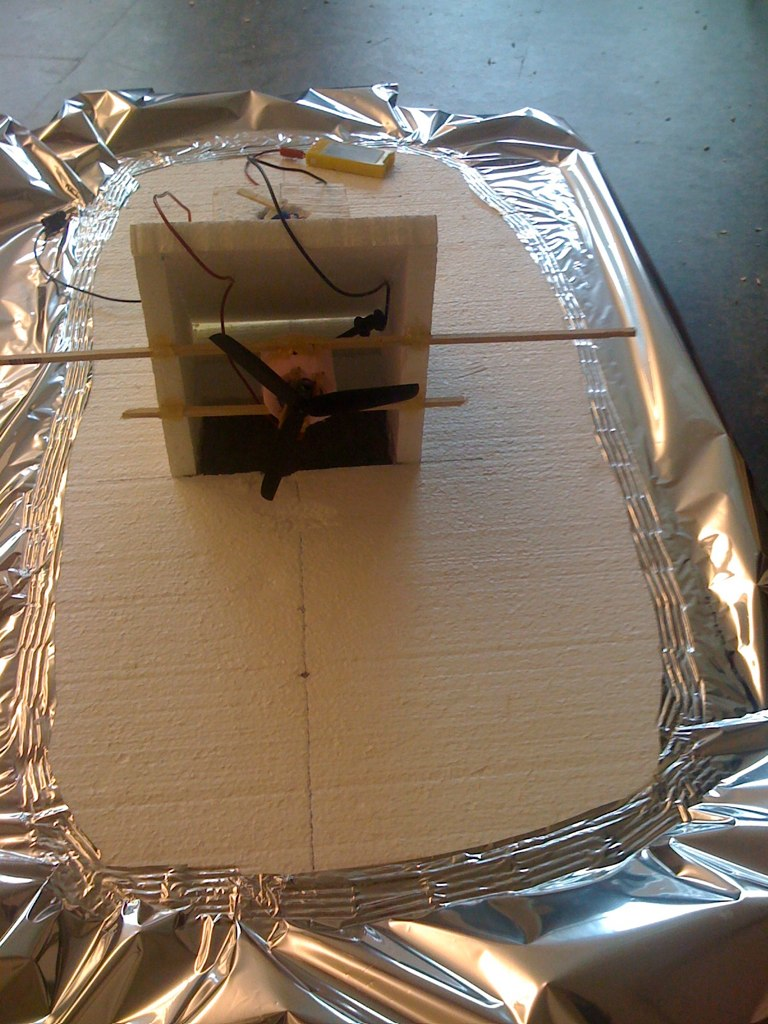
\includegraphics[width=85mm]{imageSources/lift2.png}
  \end{center}
  \caption{Hovercraft Lift II} 
  \label{lift2}
\end{figure}

To avoid ground effect, we applied full power to the lift propeller. Next, we methodically added weight to the body such that the hovercraft moved freely along the ground, but was not vastly overpowered by the fan. Keeping the vehicle as close as possible to the ground allows for the most control over the hovercraft's direction.

\subsubsection{Thrust and Control}

The following two figures show the first design we had chosen to provide the vehicle with thrust. The two differential motors were mounted at the rear, and were spaced fairly close together.

\begin{figure}[h]
  \begin{center}
    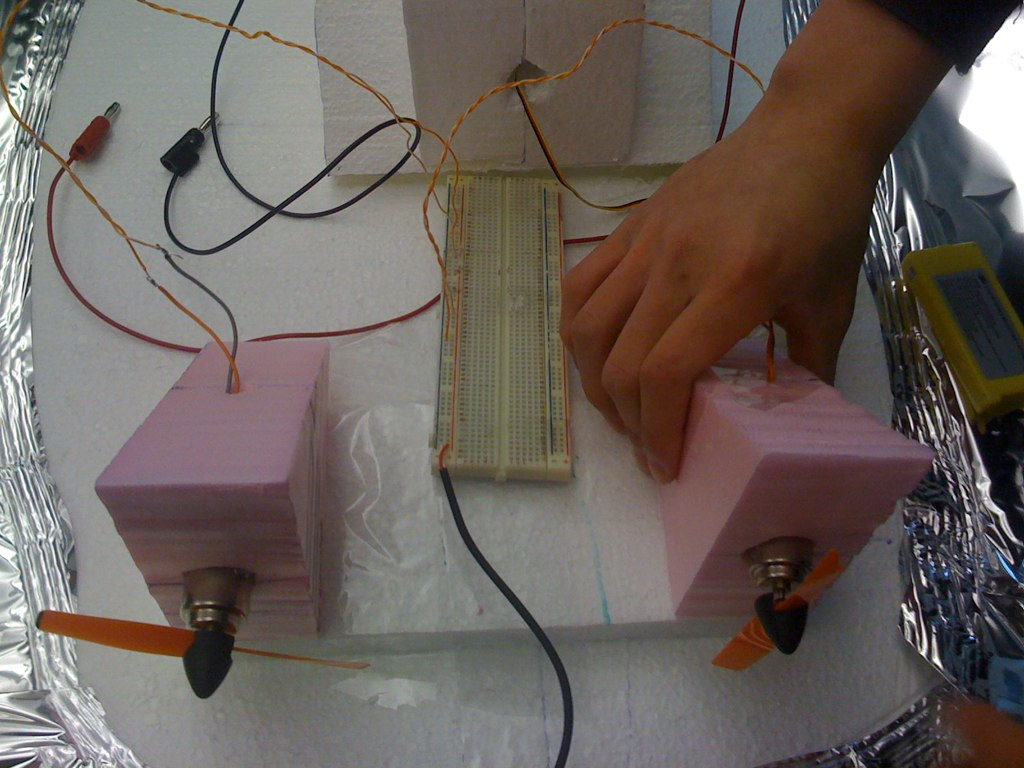
\includegraphics[width=85mm]{imageSources/thrustControl1.png}
  \end{center}
  \caption{Hovercraft Thrust and Control I} 
  \label{thrustControl1}
\end{figure}

\begin{figure}[h]
  \begin{center}
    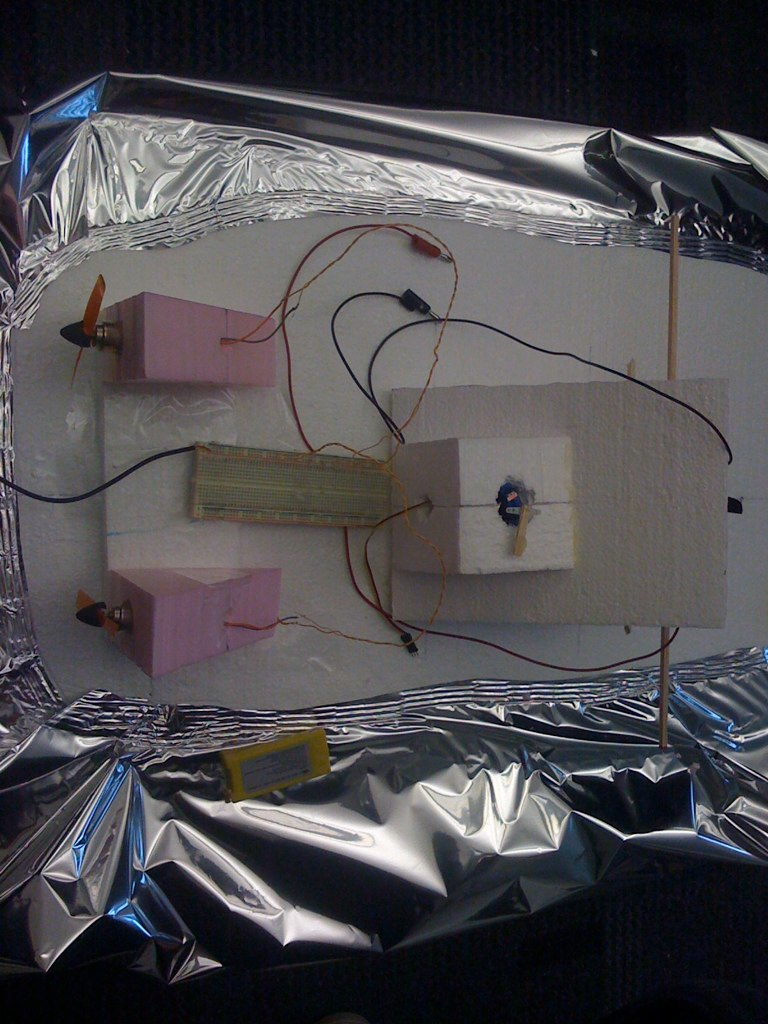
\includegraphics[width=85mm]{imageSources/thrustControl2.png}
  \end{center}
  \caption{Hovercraft Thrust and Control II} 
  \label{thrustControl2}
\end{figure}

We decided to change this design. By placing the motors as far apart as possible, maximum torque could be achieved. The analogy is as follows. Consider the act of opening a door. It is much easier to open a door if you push on the edge furthest from the hinges, because you can generate much more torque. The same goes for our hovercraft. Ideally the centre of rotation (the hinge) is in the centre of the hovercraft. By placing the motors as far away from this centre, we will create the most rotational torque and the craft will be easily controlled \cite{831309}.

\subsection{Design Problems and Future Considerations}
The following subsections describe the most challenging problems we encountered as the hovercrafts took shape.  

\subsubsection{Shape}
Our hovercraft is oval-shaped with a length to width ratio of 3:2. The first problem we encountered with this shape was that it was hard to evenly wrap our mylar around the soft corners. The mylar creased around the corners, and stuck out unevenly, often hanging down enough to provide friction for the hovercraft, creating a pivot point when we tried to move the hovercraft around. We had to make extra cuts, and then iron and glue the corners to prevent this. A hovercraft with sharper edges may take significantly less mylar tuning, and we haven't found speed to be a major issue, so the fact that square edges may reduce the aerodynamics of the hovercraft may not be as significant an issue as we thought.

\subsubsection{Weight Distribution}
Our fan blows air parallel to the ground, and we have a Styrofoam encasing around the fan directing the air down into the hovercraft base, with a single hole at the bottom of the hovercraft in the center. As mentioned above, we tried to seal the mylar around the edges of the hovercraft so that it was air-tight. We cut a Styrofoam circle that had a diameter just slightly bigger than that of the fan, and placed it even with the edge of the fan, in order to get the maximum possible amount of air intake, and prevent as little air as possible from escaping. Our fan motor is large, and is able to easily lift our hovercraft, and with this design we haven't come across any lift-related issues. The main problem we encountered having a single large fan is that it is being held up by the small square Styrofoam encasing, under 20cm in length. The fan makes up a significant portion of the overall weight of our hovercraft, and the weight distribution is all in the very center of the hovercraft. Because a large amount of the weight is in the very center, our hovercraft can easily tip, allowing air to flow out from the bottom of one side, resulting in the hovercraft gliding across the floor, or spinning.

\begin{center}
  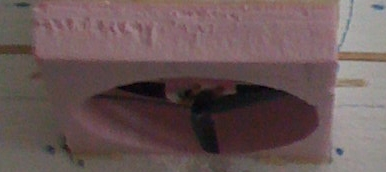
\includegraphics[width=85mm]{imageSources/weightDistro1.png}
\end{center}
\captionof{figure}{Weight Distribution I} 
\label{weightDistro1}

\begin{center}
  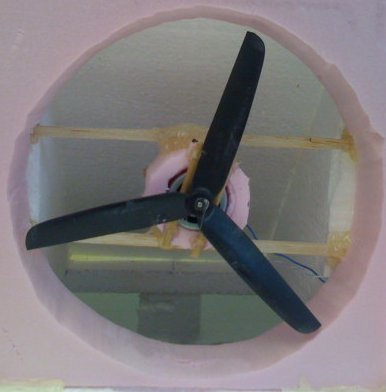
\includegraphics[width=85mm]{imageSources/weightDistro2.png}
\end{center}
\captionof{figure}{Weight Distribution II} 
\label{weightDistro2}

If the hovercraft moves around at all when just the lift fan is on, then it is extremely hard to control with the joystick. We initially hoped we could counterbalance this with software code, and shifted the power of the thrust motors on the side of the hovercraft accordingly. This took a lot of fine-tuning, and the hovercraft still was extremely hard to control, as air always seemed to be leaking from a different side, depending on the hovercraft's current movement direction and the forces exerted by the fans.

By placing weight around the edges of the hovercraft, we can greatly reduce the movement of the hovercraft when just the lift fan is on. The problem was that when enough weight was placed around the perimeter of the hovercraft that it remains motionless when the thrust motors are off, the fans had trouble moving the hovercraft forward or backward even at full power. As we took weight off, the motors could control the hovercraft more, but with less weight balancing the hovercraft, it again moves and spins uncontrollably.

\subsubsection{Turning Pivot}
We originally had our motors placed at the back end of our hovercraft, as shown in the image below. We found that the turning pivot of the hovercraft is directly inbetween where the two thrust motors are placed. With the turning pivot at the back end of the hovercraft, the turning radius of the center of the hovercraft is equal to about half of the hovercraft's length (~90cm), and it was a awkward to control the hovercraft correctly. 

\begin{center}
  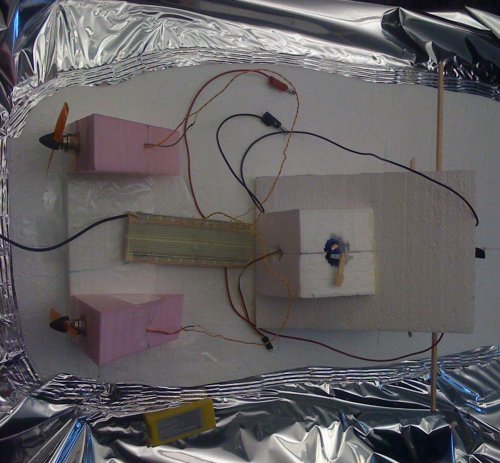
\includegraphics[width=85mm]{imageSources/turningPivot1.png}
\end{center}
\captionof{figure}{Turning Pivot I} 
\label{turningPivot1}

We shifted our thrust motors so that the fan blades were at the very center of our hovercraft. This allowed the hovercraft to have much tighter turns, and reduced our turning radius so that the hovercraft's pivot was right at the center of the hovercraft. We found controlling the hovercraft was much more intuitive this way.

\begin{center}
  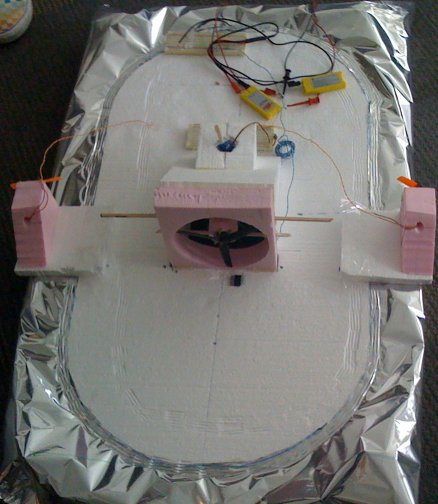
\includegraphics[width=85mm]{imageSources/turningPivot2.png}
\end{center}
\captionof{figure}{Turning Pivot II} 
\label{turningPivot2}

\subsubsection{H-bridge}
As mentioned above, one of the challenges that we encountered was that we were not getting enough power to our thrust motors. This lack of thrust was making it nearly impossible to accelerate in either direction. In the initial testing of our hovercraft design, we connected the thrusting motors directly to the 7 volt power source. In this experiment, the craft moved forward at a very quick speed over both the smooth linoleum floor and the carpet.

When testing our H-Bridge independently, it seemed like their was sufficient power being supplied to the thrust motors. Once we had the H-bridge and motors connected through the bread-board, along with the radio, and other components, the hovercraft hardly moved. The fans were moving much too slowly to accelerate our hovercraft. Our initial hypothesis was that there was not enough voltage being supplied to the H-Bridge. To solve this problem, we tried to connect an extra battery to one side of the bread-board to power the H-Bridge side, and another to control the other components on the bread-board. This solution did not seem to affect the thrust motors' power at all, as they still did not spin fast enough to accelerate our hovercraft.

After reading the documentation about the L293D H-Bridge, we found that it can only handle 1.5A maximum. At this point we tried a higher amperage H-Bridge. Again, when we wired the H-Bridge up independently, the motors spun very well, and significantly faster than with the previous L293D H-Bridge. Again, when we tested it with the rest of our components, the motors seemed to jitter, sometimes spinning as powerfully as we needed, but very irregularly. We thought this irregularity was due to a faulty H-Bridge, so we moved back to the L293D H-Bridges, that we were sure functioned correctly. As the 1.5A maximum was the limiting factor with the L293d H-Bridges, we decided to wire them in parallel. At 5 volts, this solution gave the fans almost enough power to control the hovercraft sufficiently. Unfortunately, when we used 7 volts, again the power shifted irregularly. Another problem was that we were using over 30 of the bread-boards 67 pins for our H-Bridges and Inverters alone, not leaving enough room for the other necessary components. We later found out that you can simply `piggy-back' the H-bridges, by soldering them on top of one another. This would solve the lack of pins issue. We have also since found out that the irregular power issues were caused because of the H-Bridges becoming too hot and shutting off. Attaching a heat-sink solves this problem, as we will discuss below, so two L293D H-Bridges may be a very viable option!

\begin{center}
  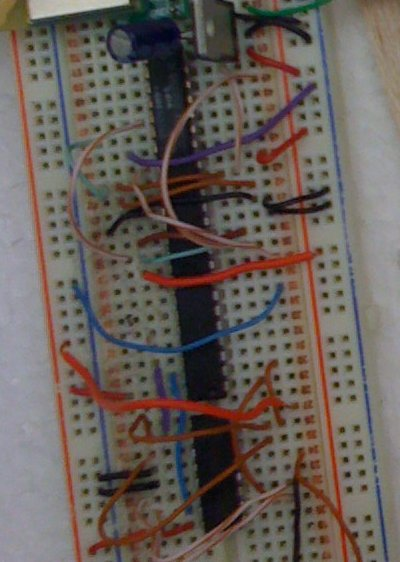
\includegraphics[width=85mm]{imageSources/designProblemsHBridge1.png}
\end{center}
\captionof{figure}{H-bridge Wiring Alternative I} 
\label{HbridgeWiring}

\begin{center}
  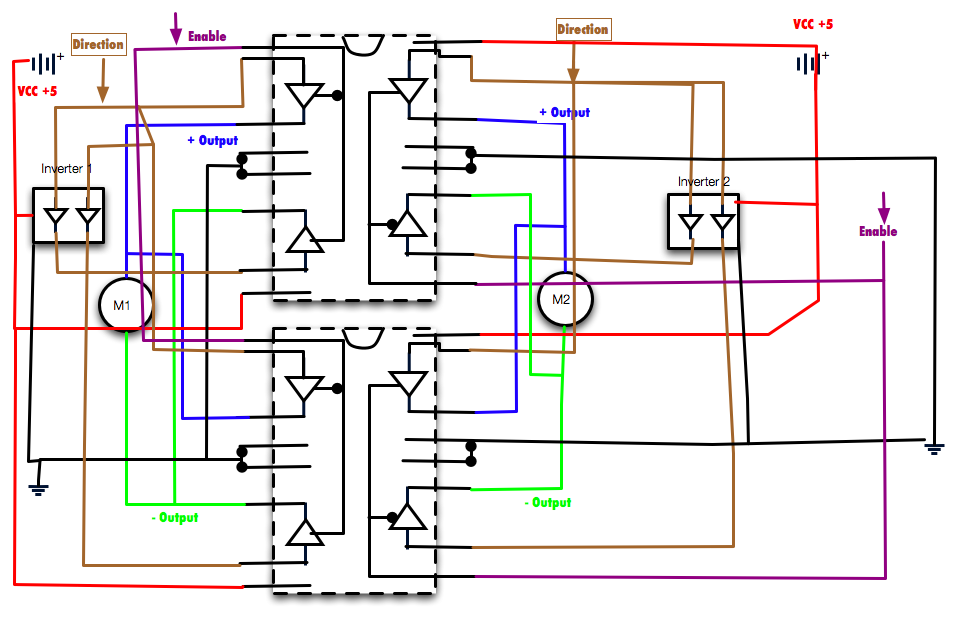
\includegraphics[width=85mm]{imageSources/designProblemsHBridge2.png}
\end{center}
\captionof{figure}{H-bridge Wiring Alternative II} 
\label{HbridgeWiring2}

At this point, we were supplied another high-amperage H-Bridge, so we went back to work on it. The new H-Bridge we were supplied also had an attached heat-sink. We were informed that the heat-sink would prevent the H-Bridge from becoming too hot and temporarily shutting off. With the heat-sink, the motors were getting enough power to successfully control the hovercraft, and the heat-sink prevented the irregular shifts in power caused by the H-Bridge shutting off.

\begin{center}
  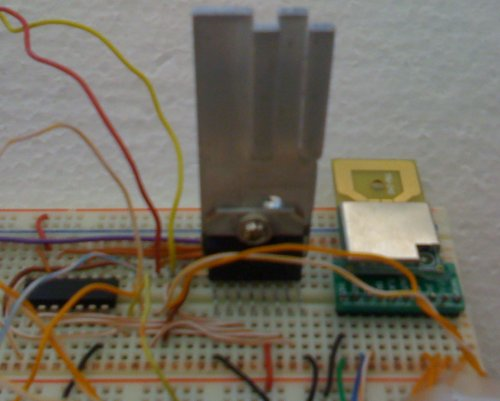
\includegraphics[width=85mm]{imageSources/designProblemsHBridgeHeatsink.png}
\end{center}
\captionof{figure}{H-bridge Heatsink} 
\label{HBridgeHeatsink}

\subsubsection{Joystick}
\label{sec:JoystickConst}
As the joystick we were supplied was seemed to produce different results every day that we tested it, and would not stay centered, it was very difficult to set-up our code to produce consistent results. We resorted to getting a new joystick that had not yet been modified to connect and work with the AT90. We took apart our new joystick, and found that it was currently using three potentiometers. One of the potentiometers was for the X position of the joystick, another was for the Y position, and the third was for the position of a dial on the base of the joystick. These potentiometers were connected so that the amount of current was determined by the position of the joystick, or the dial.

A potentiometer is a resistor with three terminals: a ground, an input, and an output (the wiper). There is a knob connected that can be spun, and as the knob is turned, the middle pin reads the voltage, and will output a reading that is the difference between ground, (zero) and the value of the input (in our case VCC).

\begin{center}
  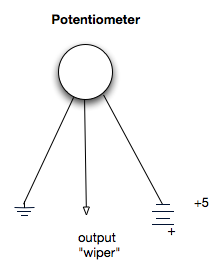
\includegraphics[width=85mm]{imageSources/joystickPotentiometer.png}
\end{center}
\captionof{figure}{Joystick Potentiometer} 
\label{joystickPotentiometer}

We decided to remove the potentiometer at the base of the joystick and simply control the hovercraft with the X- and Y-coordinates. We then were required to modify how the other two potentiometers were connected so that the amount of voltage was determined by the position of the joystick. To do this we grounded one side of the potentiometer, and connected power to the other. The middle connection was then connected through the serial port as output. Our current implementation outputs all three values at the base station, and sends them to the hovercraft, We may end up using the dial at the base of the joystick to control a ``side-stepping'' fan we could connect to the hovercraft that blows air perpendicular to the other fans. This would prevent the hovercraft from having to zig-zag down a hallway, as this fan could blow air toward the close wall to ``side-step'' the hovercraft away from the wall, without having to make an actual turn.

\begin{center}
  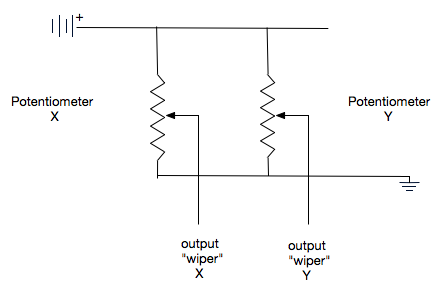
\includegraphics[width=85mm]{imageSources/potentiometerSchematic.png}
\end{center}
\captionof{figure}{Joystick Potentiometer Schematic} 
\label{potentiometerSchematic}

Once the casing was replaced on the joystick, the readings from the board, when the joystick was connected to 5 volts of regulated power, are displayed in the table below.

\begin{table}
\caption{Joystick Voltage for Direction}
\begin{center}
\begin{tabular}{ c c }
  Position & Reading (volts) \\
  \hline
  Forward & 3.76 \\
  Middle & 2.278 \\
  Backward & 0.633 \\
\end{tabular}
\end{center}
\label{voltagePotentiometerTable}
\end{table}

\subsubsection{Next Prototype}
In our next prototype, we will try and spread out the weight distribution of our center fan. This will reduce the amount of weight needed to place around the perimeter to balance the hovercraft, so the motors will be powerful enough to move the hovercraft. Now that we have our wiring completed, and are sure of the number of batteries, chips, fans, and bread-boards we will use, we can also plan a new design that takes into consideration their weights as well. Our large lift fan has always easily lifted our hovercraft, but we have found that it drains batteries quickly, our next design will also be a smaller hovercraft size, and therefore we will also use a smaller lift fan.
